%%%%%%%%%%%%%%%%%% USAGE INSTRUCTIONS %%%%%%%%%%%%%%%%%%
% - Compile using LuaLaTeX and biber, unless there is a particular reason not to. Do not use the older LaTex/PDFLaTeX or BibTeX. (The fonts won't work correctly.)
% - Font and the report 'year' must be specified when all \documentclass or the template won't work correctly. (There's no error checking/default cases!)
% - For best performance save images/graphics as PDF files, not as png/jpg/eps. This makes no difference to how images are inserted using \includegraphics.
% - As many further packages as wanted can be loaded. Below are just an example set. Note that template itself loads a number of packages, including hyperref.
% - References are handed using biblatex.
% - Link to the presentation of theses policy: https://documents.manchester.ac.uk/DocuInfo.aspx?DocID=2863



%%%%%%%%%%%%%%%%%% META DATA SETUP %%%%%%%%%%%%%%%%%%
% This is where the document title and author are set. Other details for the title page are set later
% Note that if/when you edit these you may need to 'Recompile from scratch' to get the changes to display in the PDF. (In Overleaf, select the down arrow to the right of the 'Recompile' button)
\begin{filecontents*}{\jobname.xmpdata}
    \Title{COMP30040 Report} 
    \Author{10826115} % should be student number rather than name to help with annoymous marking
    \Language{en-GB}
    \Copyrighted{True}
    % More meta-data fielda can be added here if wanted, see https://ctan.org/pkg/pdfx?lang=en for fields
    \end{filecontents*}
    
    
    %%%%%%%%%%%%%%%%%% DOCUMENT SETUP %%%%%%%%%%%%%%%%%%
    \documentclass{uom_eee_dissertation_casson} 
    
    
    %%%%%%%%%%%%%%%%%% PACKAGES AND COMMANDS %%%%%%%%%%%%%%%%%%
    
    % Packages
    \usepackage{graphicx,psfrag,color} % for postscript graphics files
    \graphicspath{ {./images/} }
    \usepackage{amsmath}               % assumes amsmath package installed
    \allowdisplaybreaks[1]           % allow eqnarrays to break across pages
    \usepackage{amssymb}               % assumes amsmath package installed 
    \usepackage{url}                   % format hyperlinks correctly
    \usepackage{rotating}              % allow portrait figures and tables
    \usepackage{multirow}              % allows merging of rows in tables
    \usepackage{lscape}                % allows pages to be typeset in landscape mode
    \usepackage{tabularx}              % allows fixed width tables
    \usepackage{verbatim}              % enhanced version of built-in verbatim environment
    \usepackage{footnote}              % allows more control over footnote environments
    \usepackage{float}                 % allows H option on floats to force here placement
    \usepackage{booktabs}              % improve table line spacing
    \usepackage{lipsum}                % for adding dummy text here
    \usepackage[base]{babel}           % for proper hypthenation in lipsum sections
    \usepackage{subcaption}            % for multiple sub-figures in a single float
    % Add your packages here
    
    % Optional: for adding alt-text to images:
    %\usepackage{pdfcomment}            % for alt text for accessibility
    % Then to add images use:
    % \pdftooltip{\includegraphics[width=0.5\textwidth]{image.pdf}}{Alt-text here}
    % This makes the text in the image non-select-able though (assuming it's a vector file)
    
    % Custom commands
    \newcommand{\degree}{\ensuremath{^\circ}}
    \newcommand{\sus}[1]{$^{\mbox{\scriptsize #1}}$} % superscript in text (e.g. 1st)
    \newcommand{\sub}[1]{$_{\mbox{\scriptsize #1}}$} % subscript in text
    \newcommand{\sect}[1]{Section~\ref{#1}}
    \newcommand{\fig}[1]{Fig.~\ref{#1}}
    \newcommand{\tab}[1]{Table~\ref{#1}}
    \newcommand{\equ}[1]{(\ref{#1})}
    \newcommand{\appx}[1]{Appendix~\ref{#1}}
    
    
    
    %%%%%%%%%%%%%%%%%% REFERENCES SETUP %%%%%%%%%%%%%%%%%%
    
    % Setup your references here. Change the reference style here if wanted
    \usepackage[style=ieee,backend=biber,backref=true,hyperref=auto]{biblatex}
    % Note backref=true adds a page number (and hyperlink) to each reference so you can easily go back from the references to the main document. You may prefer backref=false if you need to stick strictly to a given reference style
    
    
    % Fixes which can't be applied in the .cls file
    \DefineBibliographyStrings{english}{backrefpage = {cited on p\adddot},  backrefpages = {cited on pp\adddot}}
    %  \renewcommand*{\bibfont}{\large}
    
    
    % Add more .bib files here if wanted
    \addbibresource{references.bib}
    
    
    
    %%%%%%%%%%%%%%%%%% CUSTOM MODIFICATIONS %%%%%%%%%%%%%%%%%%
    \usepackage{xcolor}
    % Define a custom quote environment
    \renewenvironment{quote}
    {
        \par\setlength{\leftskip}{10pt}
        \begin{tabular}{|p{0.9\linewidth}}  % Vertical bar on the left
        \setlength{\leftskip}{10pt}
        \itshape
    }
    {
        \end{tabular}
        \par
    }
    
    % Define a custom temp environment for placeholders, etc.
    \newenvironment{temp}
    {
        \color{red}  % Set text color to red
        \itshape     % Italicize text for further distinction (optional)
    }
    {
        \normalcolor % Reset text color
    }
    
    %%%%%%%%%%%%%%%%%% START DOCUMENT %%%%%%%%%%%%%%%%%%
    
    % Don't edit these lines, title and author are automatically taken from the document meta-data defined above
    \begin{document}
    \makeatletter
    \title{\xmp@Title}
    \studentid{\xmp@Author}
    \makeatother
    
    % Set the below yourself
    \course{Computer Science}  % "Master of Science in" is added automatically
                                                     % Our courses are: Advanced Control and Systems Engineering, Advanced Control and Systems Engineering with Extended Research, Communications and Signal Processing, Communications and Signal Processing with Extended Research, Electrical Power Systems Engineering, Advanced Electrical Power Systems Engineering, Renewable Energy and Clean Technology, Renewable Energy and Clean Technology with Extended Research
    \submitdate{2025}                                  % regulations ask only for the year, not month
    \wordcount{TODO}		                           % use \wordcount{} to set the count, \thewordcount to print in the text
    \maketitle
    
    
    %%%%%%%%%%%%%%%%%% LISTS OF CONTENT %%%%%%%%%%%%%%%%%%
    \uomtoc
    % other lists are not required, but can include \uomlof and \uomlot if really want to
    \uomlof
    \uomlot
    
    %%%%%%%%%%%%%%%%%% ABBREVIATIONS %%%%%%%%%%%%%%%%%%%%%
    \phantomsection\addcontentsline{toc}{section}{Abbreviations and Acronyms}
    \section*{Abbreviations and Acronyms}
      % ALWAYS define abbreviations on first use
    
      \begin{description}
        \item[AI] Artificial Intelligence
        \item[API] Application Programming Interface
        \item[CD] Compact Disc
        \item[CDPA] Copyright, Designs and Patents Act 1988
        \item[CNN] Convolutional Neural Network
        \item[OCR] Optical Character Recognition
        \item[ML] Machine Learning
        \item[ToS] Terms of Service
        \item[TOU] Terms of Use
        \item[UX] User Experience
      \end{description}
    
    %%%%%%%%%%%%%%%%%% ABSTRACT %%%%%%%%%%%%%%%%%%%%%%%%%%
    \begin{abstract} % put abstract here. Limit is 1 page.
      Vinyl is back!
    
    \end{abstract}%
    \clearpage
    
    
    
    %%%%%%%%%%%%%%%%%% DECLARATIONS %%%%%%%%%%%%%%%%%%
    \uomdeclarations % Don't need unless final thesis
    
    
    
    %%%%%%%%%%%%%%%%%% ACKNOWLEDGEMENTS %%%%%%%%%%%%%%%%%%
    \begin{uomacknowledgements}
    I would like to extend my gratitude to the noble mahogany tree, whose sacrifice provided not only the material for a Welsh love spoon - by which I proposed and became engaged to my beloved fiancée - but also the offcuts that found purpose in the physical interface of this project. Your contribution to both my personal and academic life has been truly invaluable.
    
    Also, to my close friend Joshua Bond’s dissertation \cite{jdbond}, which I have yet to finish reading - but I am sure it is great.
    \end{uomacknowledgements}
    
    
    
    %%%%%%%%%%%%%%%%%% SECTION 1 %%%%%%%%%%%%%%%%%%
    \section{Introduction}
    
      % Written by **Sean Bechhofer**: https://studentnet.cs.manchester.ac.uk/ugt/year3/project/projectbookdetails.php?projectid=55259
    
      % Vinyl is back! According to the [NME](https://www.nme.com/news/music/uk-vinyl-sales-2023-reach-highest-level-since-1990-3563676), UK sales of vinyl in 2023 were the highest seen since 1990. Vinyl has always remained popular among niche genres, but we are also seeing mainstream artists like Taylor Swift and Lana Del Ray releasing, and selling large volumes of albums on the format. Vinyl records have also recently been added in to the ONS "Basket of Goods and Services": a carefully selected set of items representative of the goods and services that UK consumers typically spend their money on ([ONS](https://www.ons.gov.uk/news/news/arecordrevivalthatscookingupastormvinylmusicandairfryersspintheirwayintothebasketofgoods)).
    
      % Fans of the format claim better sound reproduction, with a fuller frequency range and a "warmth" lacking in digital formats such as CD. Playing vinyl requires specialist equipment: while the ritual of putting a disc on the turntable and dropping the needle is, for some, part of the experience, it can also be seen as an inconvenience.
    
      % The aim of this project will be to develop an application that supports a blending of the physical and digital worlds. A physical artefact such as an LP is scanned using a camera. The information on the label or cover is then used to identify the release which can be played. This content could be retrieved from a streaming service such as Spotify or Apple Music, an artist site such as Bandcamp [Bandcamp](https://bandcamp.com/), or the user's own personal media library. This would then allow a user to "play" their records without a turntable. Although the audio quality may not match that of vinyl, such an application would appeal to those who like to collect vinyl for its own sake, or who appreciate the larger format artwork that comes with an old school LP. The application could run on a mobile phone or specialist hardware such as a Raspberry Pi equipped with a camera.
      % Example methods that could be used for identification of the release include bar codes, QR codes or OCR acting on label text.
    
      % For a stretch goal, the application could be extended to cover other media: the cassette tape ([Guardian](https://www.theguardian.com/music/2023/apr/20/fun-way-consume-music-why-sales-of-cassette-tapes-soaring)) is also experiencing a come back, although the [eight-track](https://en.wikipedia.org/wiki/8-track_cartridge) is unlikely to be retrieved from the dustbin of history.
      % The project should be considered as challenging. It will require integration of several technologies and some creativity.
    
    \subsection{Background and motivation}
    
    \subsection{Aims and objectives}
    
    % PROJECT PLAN?
    
    \subsection{Report structure} % ROADMAP
    
      This report consists of seven chapters:
      \begin{description}
      \item[Chapter 1] presents an introduction to the project.
      \item[Chapter 2] presents the background behind this project, ...
      \item[Chapter 3] presents details on the design ...
      \item[Chapter 4] presents details on the implementation ...
      \item[Chapter 5] presents the results ...
      \item[Chapter 6] presents an evaluation  ...
      \item[Chapter 7] presents a discussion of the conclusion, limitations, and possible improvements of the project.
    \end{description}
    
    
    %%%%%%%%%%%%%%%%%% SECTION 2 %%%%%%%%%%%%%%%%%%
    \section{Background and Literature Review} % LITERATURE REVIEW / BACKGROUND
      % [ ] summary of similar systems
      % [ ] explanations of concepts relied on later
      % [ ] advanatges and disadvantages of approaches
      % [ ] highlight problems I will improve
      % [ ] cite all references
    
      \subsection{Overview of Related Systems}
    
        Whilst the creation of a digitised turntable software is a rather novel idea, it is important to consider where this sits in the existing landscape; to understand important technologies and design decisions used in similar projects, in order to best utilise them.
      
        \subsubsection{Vinyl Systems}
            % Research into questions such as 'why do people like vinyl so much?' and 'why is it making a comeback?'. Traits distilled from this feed into later design choices (I have chosen to make a make a physical artefact with a mahogany base, because physicality and aesthetics are important the people who would potentially use this system).
    
            \begin{quote}
                ``Vinyl is back!'' \cite{bechhofervttspec}
            \end{quote}
            
            In 2023, UK vinyl sales reached their highest level since 1990 \cite{geraghty2023uk_vinyl_sales}, confirming the ongoing ``vinyl revival'' \cite{vinylRevival} (see Figure~\ref{fig:vinyl_sales}). Initially dismissed as a short-term trend when it emerged in 2008-2009, this resurgence has persisted, highlighting a renewed interest in physical music formats. Understanding the motivations behind this revival is crucial for informing design decisions, particularly from a UX perspective, as vinyl collectors constitute a key target audience.
            
            \begin{figure}[htbp]
                \centering
                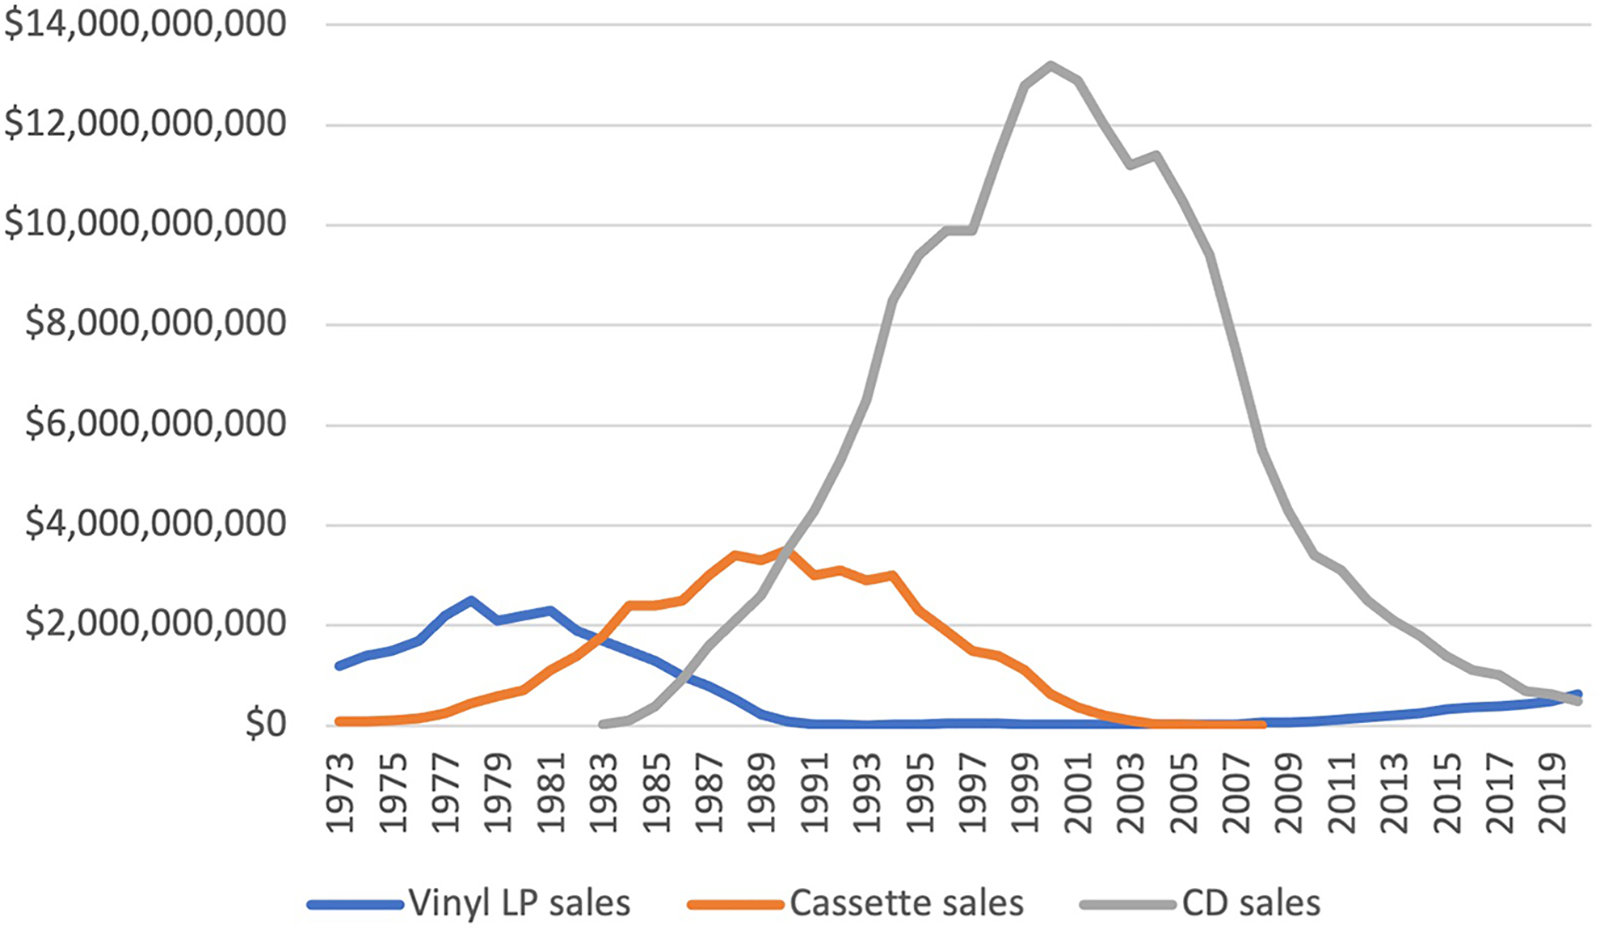
\includegraphics[width=\linewidth]{images/vinyl_sales_2023.png}
                \caption{Vinyl LP, Cassette, and CD Sales Revenue (1973–2020) \cite{vinylRevival}.}
                \label{fig:vinyl_sales}
            \end{figure}
    
    
            Although now taken for granted, records — and their predecessors, Edison's cylinders — transformed music from an ephemeral experience into a reproducible medium. Before recording technology, music was transient and confined to its place and time of performance, unable to be stored or shared beyond a live setting. While compositions could be transcribed into musical notation, each unique performance could never be heard again once it ended, unlike with visual art, where many original works from as far back as antiquity still survive \cite{jdbond}.
    
            This revolution in music consumption not only shaped the modern music industry but also cemented vinyl’s cultural significance. By making music ownable and replayable, it changed the way people engaged with it, fostering a more personal and enduring connection. Its enduring appeal, even in the digital age, suggests that its value extends beyond convenience, tapping into a deeper connection with music as a tangible experience.
    
            % Aesthetics
            \paragraph{Aesthetics and Emotional Appeal}
                % nostalgia, vibes
    
                Nostalgia plays a significant role in vinyl's resurgence. Statista data suggests the revival is primarily driven by two age groups: those aged 55+ and 25--34, with other demographics showing less engagement \cite{Gotting2021}. Older generations retain direct sentimental ties to the medium, while younger consumers are drawn to its cultural legacy.
    
                Despite the convenience of digital music, many consumers find it impersonal. In the past, music was a shared experience, often centred around a single household phonograph. Today, listeners frequently engage in isolated listening experiences \cite{historyandrevivalofvinyls}, with it being commonplace for multiple people in the same room to listen to different tracks at the same time. To an extent, music used to demand focus. You could not skip or replay a track without having to carefully reposition the needle. Some seek to reclaim the intentionality of music consumption, preferring a medium that encourages engagement rather than passive background listening \cite{Liu2020}.
    
                To many, music has become hollow- especially as music streaming services have easily monopolised the digital sphere \cite{historyandrevivalofvinyls}. Whether people are  yearning for the experiences of their past, or just a breath of `fresh air', many are turning to vinyl to do so.
    
                People are seeking community around their music and even its medium. Reddit's r/Vinyl, as of 2025, has over 2.2 million members. Whilst vinyl is still a relatively niche option, the social aspect of the internet means that, today, people are not confined to geographical constraints, and so, no matter how niche an interest is, they will be able to find like-minded people to connect to.
          
              % Ownership
              % Physicality
            \paragraph{Physicality and Ownership} % or MATERIALITY; general ethics
    
                Digital media ownership has become increasingly precarious, with consumers often purchasing revocable licenses rather than tangible assets \cite{verge2024steam_license}. This transition has upset many people, with there being many calls to bring back genuine ownership \cite{stanton2024gamers_pushback}, with legislation even being passed in California to make this fact more transparent to consumers \cite{california2024ab2426}.
    
                If a streaming vendor stops serving a particular piece of music, then that album can be lost to the public forever \cite{polygon2024cartoon_network_delisting}. However, if a consumer actually owns the physical discs or digital audio files, then they can ensure that they can listen to their audio, regardless of whatever licensing disputes may lead to the removal of digital media in the future (see \cite{bains2022lotr_strategy}).
    
                Furthermore, there are also concerns that streaming platforms often provide artists with minimal financial compensation, leading some consumers to purchase physical media as a means of direct support \cite{historyandrevivalofvinyls}. This means that there is a demographic of people who both own physical vinyls, but still make use of digital streaming services. Many even purchase physical vinyls despite not owning a device to play them on \cite{Trapp2023}. In addition, the act of gaining a physical good in support of an artist can even result in a psychological feeling of proximity to their idol \cite{historyandrevivalofvinyls}.
                
                Additionally, vinyl's finite nature contrasts with the boundless availability of digital tracks, making collections feel more meaningful and curated.
    
            % Audiophiles
            \paragraph{Audiophilia and Sound Quality}
    
                Another significant factor is the quality of the music being offered.
    
                \begin{quote}
                    \textbf{audiophile}: a person who is especially interested in high-fidelity sound reproduction. \cite{audiophile2025}
                \end{quote}
    
                % quality
                Vinyl is often perceived as superior in audio quality due to early digital compression limitations, such as the distortion issues highlighted in ``Tom's Diner'', wherein the a cappella's clean, isolated vocals revealed artifacts and distortions when encoded in early MP3 formats \cite{TODO}. Modern digital formats generally surpass vinyl in fidelity, particularly in bit depth and dynamic range. However, whilst advances in manufacturing storage drives have somewhat mitigated the need drastically to compress files, there are still valid use cases where extreme compression may be needed, such as for streaming audio on a low-quality network, which may cause the audio to sound worse than on vinyl.
    
                Additionally, as a physical format, vinyls are prone to being scratched and having physical deformities which affect the playback quality. Vinyl enthusiasts appreciate the medium’s imperfections, which are thought to add warmth and character. No two discs sounds exactly the same, whereas digital copies are utterly identical. This also creates a sense of personal ownership with vinyls - not only does the consumer own the physical disc itself, but they own their precise and unique version of it.
    
                It is important to note that many contemporary vinyl releases originate from digital masters, meaning potential losses in fidelity depend on how well an album is adapted to the format. Several inherent limitations affect vinyl playback, including: duration constraints, due to physical disk size; track sequence issues, as resolution gradually degrades towards the inner grooves; and RIAA equalisation, which alters frequency response to accommodate physical limitations of the medium \cite{engineeringvinyls}. Additionally, stereo information handling differs from digital formats, as vinyl relies on lateral and vertical groove modulation, which can introduce crosstalk and phase issues \cite{engineeringvinyls}. These factors, if not carefully managed during production, may compromise the listening experience - meaning modern tracks may often perform better in their original digital forms.
    
            \paragraph{Conclusion}
                While digital audio services offer notable convenience, the enduring vinyl revival demonstrates that many users still value tangible, nostalgic experiences. Nostalgia and charm play a crucial role in this appeal, making it essential to design with these emotional connections in mind. By combining the strengths of both physical and digital formats, a system can provide a richer, more meaningful user experience that aligns with modern consumption habits while preserving the authenticity and personal connection that vinyl enthusiasts cherish. A significant portion of consumers actively engage with both streaming services and physical media, indicating that a hybrid approach has a viable audience.
    
        \subsubsection{Image Recognition}
    
            Image recognition is the creation of software and tools which can be used to identify objects, places, people, etc. in digital images, which has existed since at least 1946 \cite{hall1979computer}. However, in this brief time, the field has undergone several drastic changes as technology has advanced \cite{imagenetclasscnn}, and is still be redefined in the present day, particularly with the arrival of machine learning approaches, with new implementations being utilised across the field (e.g. \cite{RAMPRASAD2025100556}, 2025).
    
            \paragraph{Traditional Methods}
            
                Before the advent of deep learning, image recognition primarily relied on manually crafted feature extraction techniques. Classical methods included edge detection, template matching, and statistical pattern recognition. Notable feature descriptors such as Scale-Invariant Feature Transform (SIFT), Speeded-Up Robust Features (SURF), and Histogram of Oriented Gradients (HOG) played a significant role in object detection and classification \cite{pal2001pattern}. However, these approaches were often limited by their inability to generalise across variations in lighting, scale, and occlusions. The ImageNet Large Scale Visual Recognition Challenge (ILSVRC) served as a benchmark for evaluating the effectiveness of traditional and emerging techniques \cite{russakovsky2015imagenetlargescalevisual}.
            
            \paragraph{Emergence of Convolutional Neural Networks}
            
                The introduction of convolutional neural networks (CNNs) marked a paradigm shift in image recognition. Early work, such as LeNet-5, demonstrated CNNs' potential \cite{726791}, but it was the breakthrough of AlexNet in the 2012 ImageNet competition that solidified their dominance \cite{imagenetclasscnn}. Subsequent architectures, including VGG, ResNet, and EfficientNet, further improved performance by introducing deeper networks, residual connections, and optimised convolutional layers \cite{deppcnnsforimagerecognition}. These advancements enabled significant improvements in tasks such as object detection, facial recognition, and medical image analysis.
    
                In the context of vinyl cover art recognition, CNNs offer a powerful solution for identifying album artwork despite variations in artistic style, degradation, and distortions. However, a key challenge in training CNNs for this task is the limited availability of labelled datasets. Unlike large-scale image classification datasets like ImageNet, curated datasets for album cover recognition remain relatively small. To address this limitation, data augmentation techniques—such as random cropping, rotation, colour jittering, and synthetic distortions—help improve model robustness by simulating real-world variations \cite{LIN2025102660}. There has even been research done recently into using stable diffusion techniques to facilitate fully artificial data augmentation, with generative AI \cite{Alimisis2025}.
    
            \paragraph{Multi-Headed Networks and Consensus-Based Recognition}
    
                A limitation of conventional CNN models in image recognition is their reliance on a single decision pathway, which can lead to misclassifications when dealing with visually similar or degraded images. One approach to mitigate this issue is the use of multi-headed neural networks, where multiple CNN branches extract different features and contribute to a consensus decision. This technique allows the network to assess multiple aspects of the image, such as texture, dominant colours, and key object structures, before making a final classification \cite{Zheng2017}. 
            
                By integrating multi-headed architectures with ensemble strategies, models can achieve higher classification accuracy and robustness, particularly when handling ambiguous or visually noisy inputs. This method has been successfully applied in fine-grained classification tasks and could be adapted for vinyl cover recognition by leveraging multiple specialised feature extractors that assess distinct album cover characteristics.
    
        \subsection{Legal and Ethical Considerations}
    
          The training and use of machine learning models for image classification requires the acquisition and processing of data, which, in order to effectively handle the cover art of existing albums, necessitates obtaining and using their copyrighted artworks. This raises both legal and ethical concerns, particularly regarding compliance with UK copyright law and exemptions. This section examines the legal basis for dataset usage, fair dealing exemptions, and the ethical implications of using copyrighted material in an academic AI project.
    
              \subsubsection{Copyright Law and Fair Dealing}
                  % explain copyright law
                  Under the \textit{Copyright, Designs and Patents Act 1988} \cite{cdpa1988}, creative works, including album covers, are protected from unauthorised use, reproduction, distribution, and modification.
          
                  % introduce fair dealing
                  However, UK law also provides a key exception known as Fair Dealing, which allows limited use of copyrighted material under specific conditions, although such exemptions are only granted under very specific circumstances and for a very limited scope of use. Importantly, it is not a rigid rule but a context-dependent legal doctrine, evaluated on a case-by-case basis. The law does not explicitly define what qualifies as fair dealing; instead, courts assess whether a use is reasonable and justified based on the combination of several established legal factors.
                  
                  One of the most relevant exemptions is non-commercial research, as outlined in \textit{Section 29(1)} of the CDPA:
                  \begin{quote}
                      Fair dealing with a work for the purposes of research for a non-commercial purpose does not infringe any copyright in the work provided that it is accompanied by a sufficient acknowledgement. \cite{cdpa1988}
                  \end{quote}
    
                  This indicates that non-commercial academic research can be exempt from copyright infringement if proper attribution is provided. However, the applicability of this exemption depends on further and additional factors, such as the amount of material used and its impact on the copyright holder’s market.
    
              % 1. Using a dataset to create a model
              \subsubsection{Use of Artworks in Model Training}
              
                  Album covers are protected by copyright as highly creative works. Any reproduction or modification is typically restricted without permission from the copyright holder. As such, the bar needed for fair dealings is very high when dealing with such artwork. However, training a classification model may qualify for fair dealing, provided certain conditions are met.
    
                  A key legal question is whether machine learning training qualifies as ``\textit{computational analysis}'' under \textit{Section 29A} of the CDPA, which states:
                  \begin{quote}
                      (1) The making of a copy of a work by a person who has lawful access to the work does not infringe copyright in the work provided that—
                  
                          (a) the copy is made in order that a person who has lawful access to the work may carry out a computational analysis of anything recorded in the work for the sole purpose of research for a non-commercial purpose, and
                          
                          (b) the copy is accompanied by a sufficient acknowledgement (unless this would be impossible for reasons of practicality or otherwise). \cite{cdpa1988}
                  \end{quote}
    
                  This expresses that there is a strong argument for legal use of copyrighted materials in creating a computational model which classifies data by comparisons of analytically-derived embeddings.
    
                  It is, however, important to consider whether image processing qualifies as analysis under this law or whether this interpretation is too broad, given that past applications of computational analysis have predominantly involved text, and that image processing of this kind is still relatively new. Since there is no clear legal precedent on this specific topic (with changes being in the process of being made \cite{guardian2024uk_ai_copyright}), further legal clarification over the next few years will be necessary to definitively confirm or deny its applicability to image-based AI models. But, in the time before then, it can be used as a basis.
    
                  It also reiterates the need for attribution, but, notably states that this is only required in cases where it is feasibly practical.
    
                  Given these factors, classification likely qualifies under Fair Dealing because the model does not generate new images but merely classifies existing ones. This distinction is important, especially given recent scrutiny of generative AI models like OpenAI’s \textit{DALL·E} \cite{times2025christies_ai_auction, guardian2025ai_art_auction}, which create derivative works rather than merely labelling.
    
                  None of this is clear-cut, however, as we are still in an uncertain time with the law not having been stabalised after the emergence and mass adoption \cite{bick2024rapid} of these new technologies. It is worth noting, however, that there are currently proposals for UK law the explcitly allow the use of copyrighted materials in such cases \cite{guardian2024uk_ai_copyright}, whereas, in the US, there is starting to be legal prescendent of cases winning on the basis \cite{apnews2025thomson_reuters_ai_case} of AI agents using copyrighted data.
    
              % 2. Sourcing said dataset
              \subsubsection{Legal Compliance in Dataset Sourcing}
    
                  Beyond Fair Dealing considerations, data sourcing must be legally compliant. According to \textit{Section 29A} \cite{cdpa1988}, only individuals with lawful access to copyrighted works may use them for computational analysis. Therefore, it is essential to determine how these images can be legitimately acquired.
    
                  Machine learning models must fully process training images in their entirety to generate a model. This requires the whole image to be either stored persistently (on disk) or temporarily (in memory). Even if the image is only ever stored and processed in chunks (similar to how streaming providers serve video data), the overall image is eventually processed by the model. \textit{Section 28A} outlines more leniency for cases where only temporary copies are stored, for lawful access.
    
                  It is also important to consider if entire images are required, as opposed to only sections of them. If it would be possible to achieve the desired result using only subsets of the acquired dataset, then more data would be stored and used than is justified. The legal precedent \textit{Ashdown v Telegraph Group Ltd (2002)}, highlights that:
    
                  \begin{quote}
                      The third most important factor is the amount and importance of the work that has been taken . . . in some circumstances the taking of an excessive amount, or the taking of even a small amount if on a regular basis, would negative fair dealing. \cite{tmlocad}
                  \end{quote}
    
                  Thus, ensuring only necessary data is used is critical for compliance.
    
                  % 3. ToS compliance
                  In addition to just the handling of the data, however, its source must also be considered. There are three methods by which the training dataset could be acquired: by fetching data from an API, by scraping the data from the web, or, by manually taking the required photos (either by just me, personally, or by crowd-sourcing the images). Realistically, the first two options are most practically feasible.
    
                  There are many vendors of the cover arts of music albums. Notably, music vendors (such as \textit{Spotify}) and music collection and review sites (such as \textit{Discogs}) provide the album arts in a structured format where the artworks are synchronised with the albums which they belong to. However, due to the recent boom of generative AI models - and the controversy surrounding them \cite{apnews2025mccartney_ai_warning} - many vendors have explicitly prohibited the use of their data for machine learning in their Terms of Services.
    
                  % specific examples should probably be discussed under 'Design'
                  \begin{quote}
                      Do not use the Spotify Platform or any Spotify Content to train a machine learning or AI model or otherwise ingest Spotify Content into a machine learning or AI model.
                  \end{quote} \cite{spotifyDevPolicy} (III.14)
                  \begin{quote}
                      Do not misuse the Spotify Platform, including by i. using the Spotify Platform or any Spotify Content to train a machine learning or AI model or otherwise ingesting Spotify Content into a machine learning or AI model;
                  \end{quote} \cite{spotifyDevTerms} (IV.2.a.i)
                  \begin{quote}
                      [Discogs] strictly prohibit (1) the development of any software program, including, but not limited to, training a machine learning or artificial intelligence (AI) system using the Service content
                  \end{quote} \cite{discogsToS} (LICENSE AND SITE ACCESS)
    
                  However, if a site has more permissive policies, allowing the training of AI models, then, as long as the images are handled appropriately, they can be lawfully accessed and used.
    
              \subsubsection{Ethical Considerations}
              % Even if it's legally permissible, is it ethically responsible?
              % Does it impact the commercial success of artists?
              % Transparency & attribution concerns.
    
                  Even if it is legally permissible to source and use these images, it is also important to consider whether or not it is ethically responsible. These images, at the end of the day, are the highly creative works of artists, whose livelihoods come from their creations \cite{heikkila2022ai_art}. Reproducing (by downloading) and using their works therefore cannot be done without serious moral consideration.
    
                  Most significantly, it is worth noting that this AI model is not generative (which is where most of the recent controversies stem from \cite{apnews2025mccartney_ai_warning}), and therefore, instead of producing its own artworks based off of the images fed to it, it simply classifies them by labelling them with its prediction of their corresponding album. Therefore, whilst the model is technical derived from the artist's works, the produced work is not in competition with the additional artists - unlike generative agents \cite{times2025photographer_ai_copy} - and therefore should not have a negative impact on their commercial success. If anything, it is argued that this system should benefit them, by encouraging the purchasing of physical media, and garnering instances of playing their content on a revenue-generating service.
    
                  Furthermore, as this does not share or distribute the images themselves with the users, I believe it to be even more safe, as the only artefact generated from these images are a classification system which can be used by the user, but even the numerics themselves are not made accessible to the user.
    
                  And, whilst the law allows for the exclusion for explicit attribution of all involved copyright holders, this may not be ethical. However, as this is a classification system, it arguably gives some degree of implicit accreditation to the artworks used in the training process, when the predicted label is used to redirect the user to said album.
    
              \subsubsection{Conclusion}
    
                  This section examined the legal and ethical implications of using copyrighted album covers in machine learning. Based on UK Fair Dealing exemptions in the CDPA 1988, I would argue that there is a solid grounding this project likely qualifies as a legally permissible use case, provided:
                  \begin{description}
                      \item[-] It is a non-commercial, research project.
                      \item[-] Data is lawfully acquired from permitting sources.
                      \item[-] The dataset scale and usage is minimised to strictly what is neccessary.
                      \item[-] None of the images are shared or modified. % this will need to be checked when talking about data augmentation
                  \end{description}
                  
                  From an ethical standpoint, the project is distinguishable from controversial generative AI models, as it does not replace artists’ work or impact their revenue streams. Nonetheless, transparency and attribution best practices should be followed.
    
    %%%%%%%%%%%%%%%%%% SECTION 3 %%%%%%%%%%%%%%%%%%
    \section{Design} % DESIGN / METHODOLOGY
        \begin{temp}
            What did past-Jack set out to do?
        \end{temp}
        % design diagrams!
        
        \subsection{Requirements Analysis}
            % list of requirements
        
        \subsection{System Architecture} % high-level system overview
            \subsubsection{Technology Stack}
    
                \begin{temp}
                    All of the technologies used (TS, React, bun, Python, FastAPI, etc.), and why them specifically.
                \end{temp}
        
            \subsubsection{Design Choices}
                % unique 1-1/1-many relation
                % server hardware control
                % host v. remote client
                \begin{temp}
                    Particular broad and niche design choices made, and why, such as:
                    \begin{description}
                        \item[1.] Why use a web approach for a localised device?
                        \item[2.] Why use an unorthodox 1-1 Websocket approach for client-server calls?
                    \end{description}
                    Also things such as 'point of truth handling', etc.
                    
                    Design philosophy of being an non-reliant on Spotify (or any other singular API) as possible
                \end{temp}
    
                It was decided to create a physical device that utilised online music streaming. This would allow it to have the convenience of a digital player with easy library availability and playing to the strengths of virtual playback for modern tracks, whilst still encouraging the ownership of physical mediums, and leaning into the physicality in its design and interaction mechanisms. Since the background research showed that there is an existing demographic of consumers who purchase both physical and digital copies (or subscriptions) simultaneously, this meant this design strategy would be beneficial. 
    
                In order to utilise nostalgia, the device was designed to make use of a stylish mahogany wood with brass controls. Research shows that, in one survey, wood is the most frequently cited material in nostalgic household items, appearing in 34\% of nostalgic objects (with metal second at 21\%) \cite{Skinner2022}. These materials were ubiquitous in classic mid-20th-century audio equipment, so they instantly call to mind ``the charm of a bygone era'' \cite{LookInTheAttic2024}.
        
        \subsection{Front-end}
            \subsubsection{Primary User Interface}
                % lofi designs
    
                \begin{temp}
                    - Minimal-UI approach \\
                    - Physical user interaction controls
                \end{temp}
                
            
            \subsubsection{Audio Playback}
                % Spotify Playback SDK
                % Spotify Web API
        
            \subsubsection{Remote Clients}
    
                \begin{temp}
                    - 'Remote Control' UI from an external device (mobile, etc.)
                    
                    - Gains that this system provides: accessibility (mobility, etc), convinience, scanning of out-of-house albums, etc.
    
                    - for convineince, the need for (33-45) adapter  can be cited
                    % https://external-content.duckduckgo.com/iu/?u=https%3A%2F%2Fnotesonvinyl.com%2Fwp-content%2Fuploads%2F2022%2F04%2Fspeeds-of-the-different-record-types-1.png&f=1&nofb=1&ipt=7d1e31af8468ae7ae70f11be6bd40c897a73cf0c42aa194a5e09309f9af25945&ipo=images
                    % https://external-content.duckduckgo.com/iu/?u=https%3A%2F%2Fwww.bluescentric.com%2Fimages%2Fproduct%2Flarge%2F557_2_.jpg&f=1&nofb=1&ipt=1cd939744050d9f13eb7f581b786a2f22d3787cf30dd60c2a6975a816043546f&ipo=images
                \end{temp}
        
        \subsection{Back-end}
        
            \subsubsection{Metadata Retrieval}
                % Discogs API
                % assert Discogs ToS compliance (not used for AI) 
          
            \subsubsection{Hardware Interaction}
                % RPi
        
        \subsection{Machine Learning Model Design}
            \subsubsection{Dataset Collection}
                % use of CoverArtArchive
        
            \subsubsection{Model Architecture}
        
        \subsection{Security Considerations}
            % handling of auth tokens (transient)
            % off-handing of persistence tasks
            % network hosting
            % option of same-user or any-user controls
            % API compliances
        
        \subsection{Testing Methodology}
    
            \begin{temp}
                Design of tests and evaluations; plan for unit testing, model evaluation, etc.
                
                Does the system satisfy that physical and aesthetic desires of that the vinyl trend appeals to, whilst still offering functional convenience over original systems?
            \end{temp}
            
            \subsubsection{Validation of Effectiveness}
                \begin{temp}
                1. Model performance (formal model evaluation)
                2. Usability (user feedback)
                
                3. Code robustness (Unit Tests, etc.)
                \end{temp}
        
        \subsubsection{Validation of Affectiveness}
            \begin{temp}
                User feedback on aesthetics
            \end{temp}
    
    
    %%%%%%%%%%%%%%%%%% SECTION 4 %%%%%%%%%%%%%%%%%%
    \section{Implementation}
        \begin{temp}
            Details realised in practice, decisions made, etc.\\
            Challenges encountered, how addressed, etc.
        \end{temp}
        % details realised in practice
        % challenges, and how overcame
        % code-level or system-specific decisions, optimizations, or trade-offs
        % integration
    
        \subsection{Front-end}
            \subsubsection{Challenges Encountered}
                \begin{temp}
                    1. Switch to minimal UI mid-production
                    2. Responsive / wholeness tradeoff (do we wait for the centre label before playing the audio?)
                    3. Media codec, DRM, etc. issues specific to Ubuntu/aarch64 OS.
                \end{temp}
    
        \subsection{Back-end} % maybe Front/Back should just merge to software, here
            \subsubsection{Challenges Encountered}
                \begin{temp}
                    1. Change of auth flow, due to 'remote client' introduction
                    2. Removal of barcode detection form spec, due to camera limitations
                    3. \cite{spotify2025security}
                \end{temp}
    
        \subsection{Hardware}
            \subsubsection{Challenges Encountered}
                \begin{temp}
                    1. Lack of 'Measure twice, cut once' methodology (fried GPIO pin; overstrained motor driver)
                    2. Voltage issues
                    3. Overheating (throttling) issues
                \end{temp}
    
      \subsection{Machine Learning Model}
    
            \begin{temp}
                cite \cite{Mitchell_2019}
            \end{temp}
      
            \subsubsection{System Integration}
                \begin{temp}
                    Practice-driven discoveries, such as 'how much is not too much' when it came to model   architecture and the Pi's specs.
                \end{temp}
            
            \subsubsection{Challenges Encountered}
    
                \begin{temp}
                    Internet Archive downtime!
                \end{temp}
    
    
    %%%%%%%%%%%%%%%%%% SECTION 5 %%%%%%%%%%%%%%%%%%
    \section{Results} % edit section heading as appropriate
        \begin{temp}
            What was actually produced?
        \end{temp}
        % results of soft/hardware testing
        % screenshots of UI / program output
        \subsection{Software Artefact}
        
        \subsection{Hardware Artefact}
    
    %%%%%%%%%%%%%%%%%% SECTION 6 %%%%%%%%%%%%%%%%%%
    \section{Evaluation}
        % does it do what it is supposed to do?
        % how well?
        % how well against others?
        \subsection{Machine Learning Model Performance}
        
        \subsection{User Experience}
        
        \subsection{Comparison with Existing Systems}
        
        \subsection{Ethical Implications}
    
    
    %%%%%%%%%%%%%%%%%% SECTION 7 %%%%%%%%%%%%%%%%%%
    \section{Conclusions and future work} % edit section heading as appropriate
        \subsection{Conclusions}
          % summarise results
          % achieved aims?
          % improvements!
        
        \subsection{Future work}
          % ideas for further work
          % big ideas; what could be done with my project?
    
    
    %%%%%%%%%%%%%%%%%% REFERENCES %%%%%%%%%%%%%%%%%%
    %\clearpage % uncomment to start on a new page if wanted
    \printbibliography[title={References},heading=bibintoc] % a single list of references for the whole thesis
    
    
    
    %%%%%%%%%%%%%%%%%% APPENDICES %%%%%%%%%%%%%%%%%%
    \begin{uomappendix} 
        % screen dumps of UI
        % important but large results
        \section{Project outline}
    
            \begin{temp}
                Project outline is a required appendix. Put here.
            \end{temp}
            
            Vinyl is back! According to the \href{https://www.nme.com/news/music/uk-vinyl-sales-2023-reach-highest-level-since-1990-3563676}{NME}, UK sales of vinyl in 2023 were the highest seen since 1990. Vinyl has always remained popular among niche genres, but we are also seeing mainstream artists like Taylor Swift and Lana Del Rey releasing and selling large volumes of albums on the format. Vinyl records have also recently been added into the ONS "Basket of Goods and Services": a carefully selected set of items representative of the goods and services that UK consumers typically spend their money on (\href{https://www.ons.gov.uk/news/news/arecordrevivalthatscookingupastormvinylmusicandairfryersspintheirwayintothebasketofgoods}{ONS}).
            
            Fans of the format claim better sound reproduction, with a fuller frequency range and a "warmth" lacking in digital formats such as CD. Playing vinyl requires specialist equipment: while the ritual of putting a disc on the turntable and dropping the needle is, for some, part of the experience, it can also be seen as an inconvenience.
            
            The aim of this project will be to develop an application that supports a blending of the physical and digital worlds. A physical artefact such as an LP is scanned using a camera. The information on the label or cover is then used to identify the release which can be played. This content could be retrieved from a streaming service such as Spotify or Apple Music, an artist site such as \href{https://bandcamp.com/}{Bandcamp}, or the user's own personal media library. This would then allow a user to "play" their records without a turntable. Although the audio quality may not match that of vinyl, such an application would appeal to those who like to collect vinyl for its own sake, or who appreciate the larger format artwork that comes with an old school LP. The application could run on a mobile phone or specialist hardware such as a Raspberry Pi equipped with a camera.
            
            Example methods that could be used for identification of the release include barcodes, QR codes or OCR acting on label text.
            
            For a stretch goal, the application could be extended to cover other media: the cassette tape (\href{https://www.theguardian.com/music/2023/apr/20/fun-way-consume-music-why-sales-of-cassette-tapes-soaring}{Guardian}) is also experiencing a comeback, although the \href{https://en.wikipedia.org/wiki/8-track_cartridge}{eight-track} is unlikely to be retrieved from the dustbin of history.
            
            The project should be considered as challenging. It will require integration of several technologies and some creativity.
        
        \section{Risk assessment}
            \begin{temp}
                Risk assessment is a required appendix. Put here.
            \end{temp}
    
        \section{Model Card}
            \begin{temp}
                TODO
            \end{temp}
        
        %\section{Other appendices as necessary}
    \end{uomappendix}
    
    
    %%%%%%%%%%%%%%%%%% END MATTER %%%%%%%%%%%%%%%%%%
    \end{document}